
\section{The Flyspeck Project}
\label{sec:flyspeck}

\begin{wrapfigure}{r}{4.2cm}
  \centering
  \vspace{-.9cm}
  \begin{tikzpicture}
    \node (s) at (0,0) {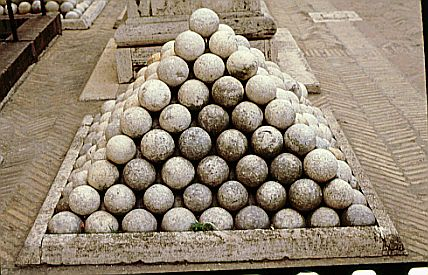
\includegraphics[width=4cm]{images/cannonballs.jpg}};
  \end{tikzpicture}
  \vspace{-1.2cm}
\end{wrapfigure}

%% alternative images are
%% http://mathworld.wolfram.com/images/eps-gif/CircleSpherePacking_800.gif
%% http://en.wikipedia.org/wiki/Image:Close-packed_spheres.jpg

The target of our case study is the Flyspeck Project, which seeks to
formally verify Thomas Hales' 2005 proof of the Kepler Conjecture.
The Kepler Conjecture asserts that the density of a packing of unit
spheres in 3 dimensions is at most $\pi/(3\sqrt{2})$, the density of the face centered
cubic and hexagonal close packings.  The conjecture, posed by Kepler
in 1611, formed part of Hilbert's 18th problem, and until its solution
was recognized as one of the most famous unsolved problems of
mathematics.

Hales' proof, completed in 1995, was not accepted immediately by the mathematical community. 
Besides its considerable length,  the proof relies essentially on computer calculations.  
The 300 pages of text and many thousands of lines of computer code made
checking the proof for errors in the referee process unusually difficult,
leading to a publication delay of nearly 10 years.  
In 2003, Hales proposed using computers to rigorously check the entire proof in
detail, including the computer code.  He dubbed this
effort the \textit{Flyspeck Project}
\footnote{The word ``flyspeck'' means, ``to examine closely''.  It was found
by Hales using a regular expression search of an English dictionary for the
expression ``F.*P.*K'', for ``Formal Proof of Kepler''}.  
The software systems used in such formalizations are called \textit{theorem provers}
or \textit{proof assistants}.
Beginning with a set of axioms and inference rules, they can,
with adequate human guidance, verify that a purported proof follows from the axioms.  
Examples of proof assistants are Isabelle\cite{Paulson:1994:Isabelle}, 
Coq\cite{Bertot:2004:CoqBook}, Mizar\cite{mizarmanual},
and HOL Light\cite{Harrison:2000:HOL-Light}. (In the rest of this paper, we use ``formalize'' to mean
that the theorem, proof or definition has been expressed in one of these
systems.)\ednote{@CL: Remove Mizar for shortening}

  Unfortunately, modern proof assistants are still far from being able to check
proofs at the level given in most journals and mathematics textbooks.  A typical
estimate is that it takes about a week to formalize a single page of mathematical
text.  Based on such estimates, Hales' expects that it will take 
around 20 man-years to complete the Flyspeck project.  
Hales is compiling a book\cite{Hales:2007:FlyspeckBook}
of lemmas from different areas of mathematics to make the formalization easier.    
That book is currently 450 pages, and contains a large number of mathematical
results used in the proof.  It covers such disperate topics
as plane, solid, and sphereical geometry, graph theory and hypermaps, single and
multivariable calculus, and plane and sphereical trigonometry.

The first steps toward a formal proof have already been taken.  Nipkow
and Bauer\cite{Nipkow:2005:Tame} proved the correctness of a
fundamental algorithm in Isabelle.  Other parts of the computer code
are being investigated, including the linear programming and global
optimization.  There is a project
page\cite{website:FlyspeckProjectPage} for Flyspeck hosted at
GoogleCode\cite{website:GoogleCode} that documents some of the
progress.  That page has a source repository containing the book of
lemmas, as well as the formalized definitions of some important
functions and inequalities.  Yet while important work has already been done,
the project is still in its infancy.  

Flyspeck is a particularly appealing as a use case
for a semantic wiki approach. It
involves both highly formal and semi-formal mathematical knowledge.   
The original proof contains descriptive and motivating yet informal text that would
be difficult to present in a strictly formal setting.
Finally, its purpose is to develop a scientific document---a formal proof of the Kepler
conjecture--- and to communicate this proof to the public.  Its large extent and the
required manpower suggest ``crowdsourcing'' the workload and supporting the project
organization by social software.  For example, doing this publicly on the web will contribute to
communicating the parts of the proof already done.  We are going to investigate whether
the three conditions for successful peer production stated by Tapscott and
Williams\cite{wikinomics} will hold or can be satisfied by software support.
The conditions are
\begin{enumerate} 
\item The object of production is (immaterial) information, which
  keeps the cost of participation low.
\item We can break tasks down into small pieces\ednote{Check whether we actually show this in this paper! --CL} that can be worked
  off independently.
\item The cost of integrating the individual contributions is low.
\end{enumerate} 


Flyspeck consists of thousands of subproblems that need to be
managed such that a widely distributed user base can work
efficiently.  

\ednote{@Sean/Florian: One/two sentences about Twelf! (here or in
  some other section where it's appropriate, either workflow or flyspeck) What
  is it, why was it originally chosen? --CL}
